\documentclass[letterpaper,11pt]{article}
\usepackage[spanish]{babel}
\usepackage[utf8]{inputenc}
\usepackage{graphicx,hyperref,amsmath,amssymb,ragged2e,tabularx,multirow,natbib,bibentry,graphics,color,float}
\usepackage{listingsutf8}



	\title{Matrices de datos y imágenes en \LaTeX{}}
%\subtitle{Presentación del curso}
\author{Valentín Vergara Hidd}
%\institute[UdeC]{Universidad de Concepción}
\date{\today}
%\logo{udec}


%\setbeamertemplate{navigation symbols}{}
%\usetheme{Madrid}
%\usecolortheme{albatross}
%\usecolortheme[named=Black]{structure}\lstset{% general command to set parameter(s)

%\usefonttheme[onlymath]{serif}
%\justifying

%\usebackgroundtemplate{\scalebox{0.6}{\includegraphics[width=\paperwidth]{ko.eps}}}
%\pgfdeclareimage[height=1.2cm, width=1cm]{logo}{udec}
%\logo{\pgfuseimage{logo}}

\begin{document}
\lstset{% general command to set parameter(s)
	language=[LaTeX]TeX,
	basicstyle=\scriptsize\ttfamily, % print whole listing small
	keywordstyle=\color{cyan},
	framexleftmargin=-2pt,
	%backgroundcolor=\color{gray!10},
	frame=single,
	tabsize=2,
	%rulecolor=\color{black!30},
	title=\lstname,
	escapeinside={\%*}{*)},
	breaklines=true,
	breakatwhitespace=true,
	framextopmargin=-5pt,
	framexbottommargin=-5pt,
	extendedchars=false,
	inputencoding=utf8,
	literate={á}{{\'{a}}}1, 
	literate={é}{{\'{e}}}1,	
	literate={ó}{{\'{o}}}1,
	literate={ú}{{\'{u}}}1,
	literate={ñ}{{\~{n}}}1, 
	literate={í}{{\'{i}}}1
}

\maketitle

%\renewcommand{\listtablename}{Índice de tablas} 
%\renewcommand{\tablename}{Tabla} 

\section{Matrices de datos}

Como primer antecedente, la Matriz de Datos (Samaja, 1994), utiliza la conceptualización de Galtung y Lazarsfeld sobre el \emph{dato}. En ella, cualquier dato científico se puede descomponer en tres partes:
\begin{description}
\item[UA: ] La \emph{unidad de análisis}, que hace referencia directa a qué o quiénes proporcionan los datos. Pueden ser individuales, o de agregaciones de individuos.
\item[V: ] Variable, que se refiere a una dimensión o un aspecto de las unidades de análisis que se está observando.
\item[R: ] Valor de la variable, que se presenta como una observación particular, de una variable para una unidad de análisis en particular. 
\end{description}

Para hacer más claro lo anterior y relacionarlo con la forma en la que generalmente los sociólogos (y cualquier ciencia empírica) trabajamos con los datos científicos, Samaja vincula este trio de atributos del dato al concepto algebraico de matrices.

Al respecto, conviene recordar que una matriz es un \emph{ordenamiento} de elementos en filas y en columnas. En ese sentido, una matriz $A$ tiene la siguiente forma:

\begin{equation*}
	A = \begin{pmatrix}
		a_{11} & a_{12} & a_{13} & \ldots & a_{1m}\\
		a_{21} & a_{22} & a_{23} & \ldots & a_{2m}\\
		a_{31} & a_{32} & a_{33} & \ldots & a_{3m}\\
		\vdots & \vdots	& \vdots & \ddots & \vdots \\
		a_{n1} & a_{n2} & a_{n3} & \ldots & a_{nm}
	\end{pmatrix}
\end{equation*}
 y su \emph{tamaño} es de $n\times m$, lo que quiere decir que tiene $n$ filas y $m$ columnas.
 
 Por tanto, una matriz de datos $A_{n\times m}$ es una matriz de datos en la medida en que:
 \begin{description}
		\item[$\{1, 2, 3, \ldots, n\}$] Corresponde a las unidades de análisis (UA) de las que se compone la muestra a analizar.
		\item[$\{1,2,3,\ldots,m\}$] Son las variables (V) que se observan de las unidades de análisis.
		\item[$\{a_{11}, a_{12}, a_{13}, \ldots, a_{nm}\}$] Es el valor de la variable (R), lo que implica la intersección entre una variable y un caso determinado. Dicho de otra forma, es el valor de una variable para una unidad de análisis en observación.
 \end{description} 
 
 La ventaja de la conceptualización anterior es que permite trabajar con matrices de cualquier tipo de datos. Pueden ser datos de  una encuesta, fundamentalmente numéricos; o pueden también ser datos de un análisis de discurso, donde las variable son de tipo categórico y tienen valores fundamentalmente de texto. 
 
 Lo anterior se parece mucho a la forma en que estamos acostumbrados a ordenar los datos en una planilla de cálculo, como por ejemplo MS Excel. Es por esta estructura de presentación de datos en filas y columnas que muchas veces recibimos ---y también--- producimos datos en estas planillas. Las últimas versiones de los software de planillas de cálculo usualmente incorporan además algunas funciones estadísticas, que en teoría posibilitan análisis estadísticos. Sin embargo, no vamos a explorar con detalle estas opciones, puesto que la herramienta más adecuada para los análisis estadísticos generalmente es un lenguaje de programación más flexible y orientado a objetos, como R. 
 
 \subsection{Matrices de datos en planillas de cálculo}
 
 Generalmente, en los cursos de análisis de datos se trabaja con alguna matriz de datos preparada previamente por quien organice el curso o directamente extraída de un libro de texto. El problema que veo respecto a eso es que generalmente los datos se ajustan de forma muy perfecta a lo que sea que se esté enseñando. para transparentar este sesgo, para la primera actividad de esta clase vamos a trabajar con datos simulados.
 
 Las indicaciones para preparar esta matriz de datos simulados, que por ahora sólo incluirá variables numéricas, son las siguientes:
 \begin{enumerate}
 	\item Abra un libro en blanco y en la primera hoja, en la primera celda de la primera columna (A1) escriba ID. Esta será la variable de identificación de los casos.
 	\item Cree números correlativos del 1 al 100. Esto significa que la matriz de datos simulada tendrá 100 UA.
 	\item la segunda columna será la edad de estas 100 UA ficticias. Para garantizar que los valores de las edades sean aleatorios, vamos a utilizar la siguiente función:
 	\begin{lstlisting}
 		=ALEATORIO(inferior;superior)
 	\end{lstlisting}
 	donde \emph{inferior} se debe reemplazar por el menor valor que se quiera en la muestra y \emph{superior} por el mayor. Como en este caso vamos a trabajar con edades, pensemos en personas de 18 a 65 años. La función quedaría así:
 	\begin{lstlisting}
 		=ALEATORIO(18;65)
 	\end{lstlisting}
 	\item La tercera variable queda a su criterio, teniendo como única indicación que tenga una distribución normal. Eso se logra de esta forma:
 	\begin{lstlisting}
 		=INV.NORM(ALEATORIO();media;ds)
 	\end{lstlisting}donde \emph{media} es el valor que se busca que tenga la distribución y \emph{ds} su desviación estándar.
 	\item Para la cuarta, quinta y sexta variable, dejo a su criterio los valores y las distribuciones de cada una de ellas. 
 \end{enumerate}
 
 \section{Gráficos en Planillas de cálculo}
 
 Para esta sección, voy a utilizar ejemplos de MS Excel 2016 para Windows y para Mac. Sin embargo, las instrucciones deberían funcionar con pocos cambios para versiones anteriores.
 
 Una forma de trabajar con una variable, es seleccionar el rango de los datos y luego en la barra superior, ir a la pestaña {\ttfamily Insertar}, para luego seleccionar el gráfico.
 \begin{figure}[H]
 \centering
 \scalebox{0.39}{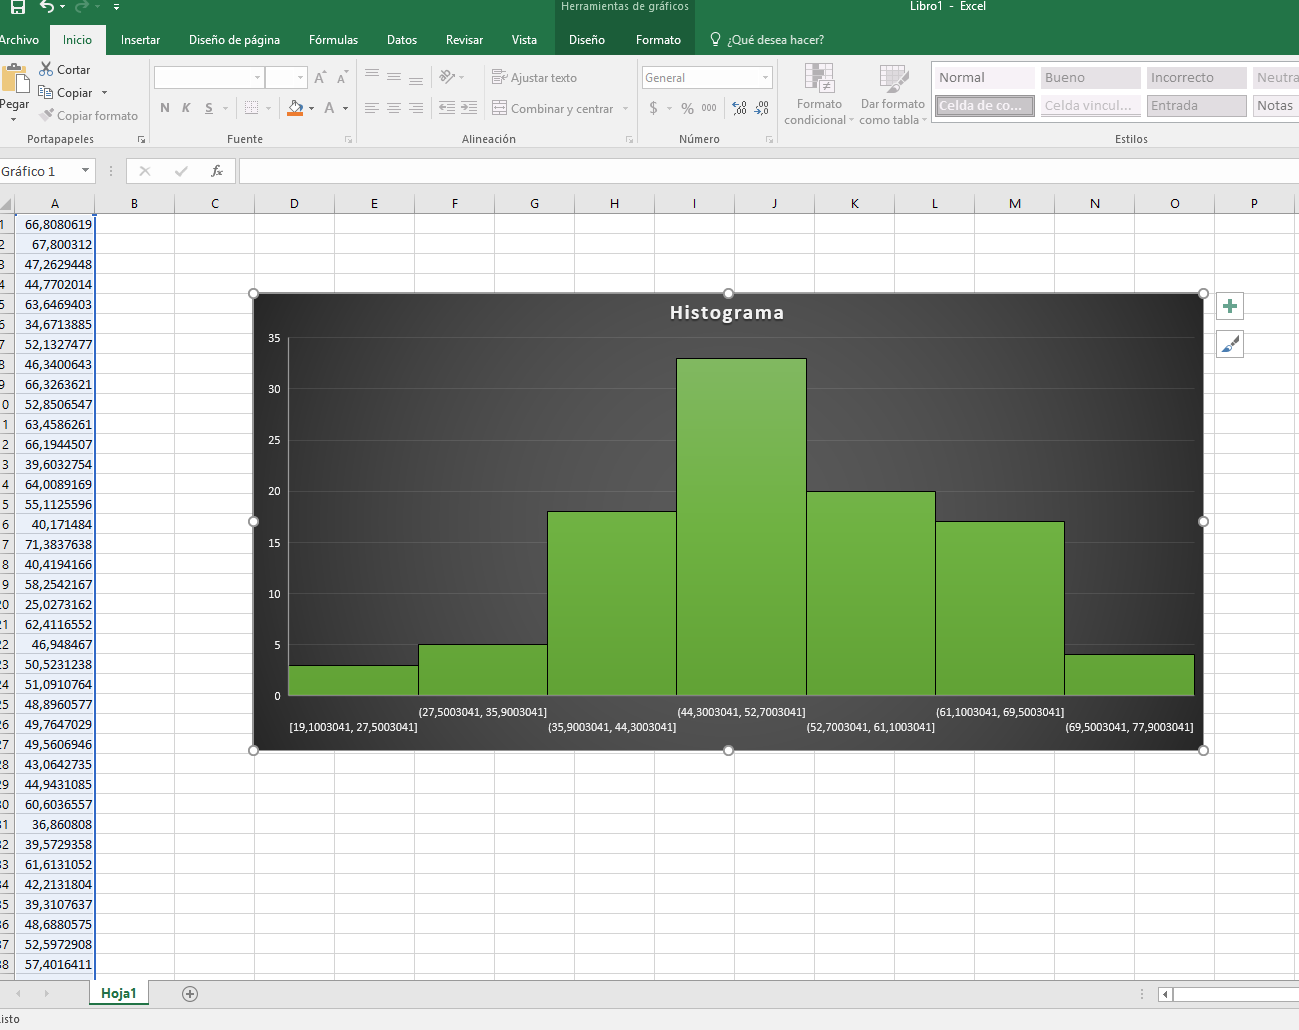
\includegraphics{2_1.png}}
 \caption{Creación de un gráfico a partir de una variable en Windows}
 \end{figure}
 
 Una vez que se tiene este gráfico, se puede copiar y pegar en el editor de imágenes que usen. Hay que hacer lo posible por guardar la imagen en formato .eps. Muchos de los software que vienen preinstalados en los sistemas operativos de amplio uso, no tienen la opción de exportar imágenes a .eps; por lo que sugiero instalar GIMP y exportar la imagen en este formato. Si no es posible, se puede trabajar con imágenes en formato .png, para lo que hay que cambiar el motor de compilación de documentos a {\ttfamily pdfLaTeX}.
 
 \begin{figure}[H]
 \centering
 \scalebox{0.49}{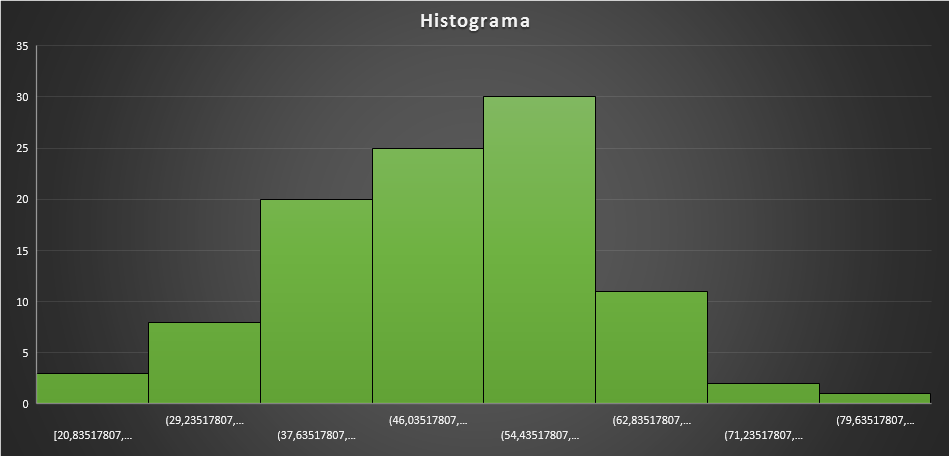
\includegraphics{2_2.png}}
 \caption{Así se ve un gráfico desde MS Excel.}
 \end{figure}
 
 Para incluir un gráfico de nube de puntos, se debe trabajar con dos variables. Para este ejemplo, simulé dos variables aleatorias con distribución normal.
 
 \begin{figure}[H]
 \centering
 \scalebox{0.32}{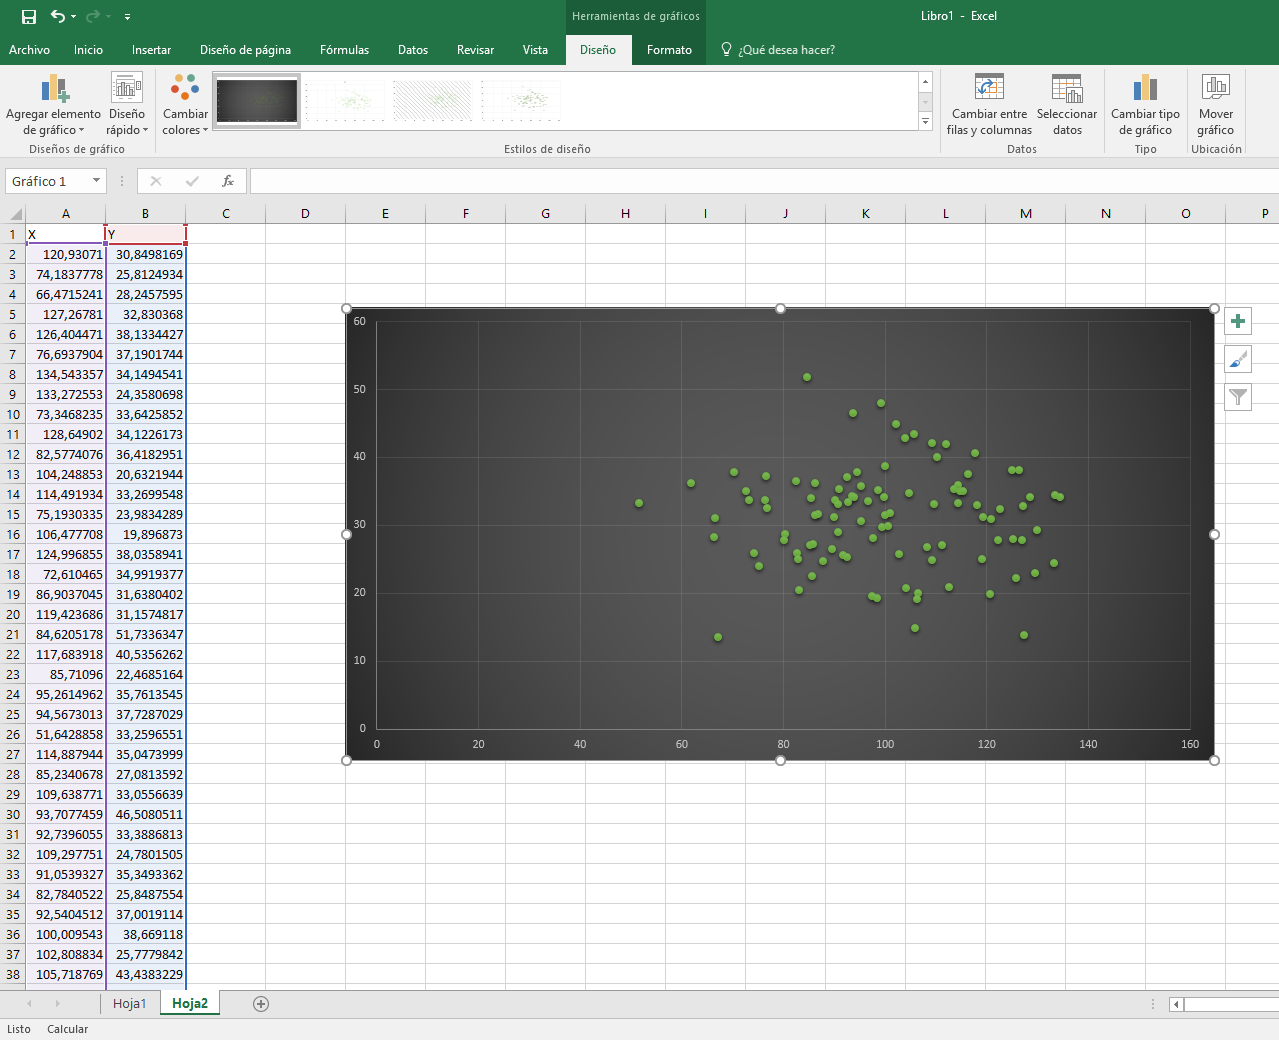
\includegraphics{2_3.png}}
 \caption{Para una nube de puntos, se deben seleccionar dos variables.}
 \end{figure}

\section{Gráficos en \LaTeX{}}
Para un adecuado manejo de gráficos, se deben cargar los siguientes paquetes.
\begin{itemize}
	\item graphicx
	\item float
	\item color
	\item hyperref
\end{itemize}

Los gráficos se incluyen en el entorno {\ttfamily figure}. Por ejemplo

\begin{lstlisting}
	\begin{figure}[H]
		
	\end{figure}
\end{lstlisting}

Notarán que hay una letra H, una opción del entorno, que indica que la imagen debe ir en el mismo lugar en el que aparece en el código. Por defecto, \LaTeX{} detecta automáticamente la mejor ubicación de la imagen, dado su tamaño y el resto del texto en el documento, por lo que podría dejarlas al final de la hoja o incluso en hojas siguientes.

Una vez dentro del entorno \emph{figure}, se pueden incluir algunas opciones, por ejemplo, usualmente agrego la siguiente instrucción:
\begin{lstlisting}
	\begin{figure}[H]
	\centering 
	\end{figure}
\end{lstlisting}

Una vez que se han introducido las instrucciones de \emph{formato} necesarias, se debe incluir la imagen, utilizando la instrucción {\ttfamily includegraphics}.

\begin{lstlisting}
	\begin{figure}[H]
	\centering
	\includegraphics{nombredelaimagen.extension}	
	\end{figure}
\end{lstlisting}

Para garantizar que lo anterior funcione, la imagen debe estar en la misma carpeta que el archivo .tex; pudiendo en la mayoría de los casos omitir la extensión. Por defecto, el motor \emph{pdfLaTeX} procesa gráficos de mapa de bits o gráficos vectorizados. Idealmente se deben preferir los últimos, puesto que tienen un mejor soporte para redimensión (hacer las imágenes más grandes o más pequeñas).

\begin{table}[H]
	\centering
	\caption{Tipos de gráficos que se pueden insertar en \LaTeX{}}
	\begin{tabular}{ll}
	\hline \hline
	Mapa de bits		& Vectorizados\\
	\hline
	.png			& .eps	\\
	.jpg			& .pdf  \\
	\hline \hline 
	\end{tabular}
\end{table}


\subsection{Redimensionar Imágenes}

El primer intento de incluir una imagen en un documento \LaTeX{} casi siempre resulta ser un fracaso. Esto porque por lo general queda demasiado grande para ajustarse a las dimensiones que necesitamos; o bien porque es muy pequeña para que resulte legible. Para esto, se puede utilizar la instrucción {\ttfamily scalebox}, seguida de una proporción\footnote{No olvidar que una proporción es un número real que se encuentra entre 0 y 1}. Por ejemplo, si queremos adjuntar una imagen en .eps que se llame \emph{test}, pero es muy grande y sólo nos sirve si la redimensionamos a la mitad de su tamaño, el código \LaTeX{} se debería ver así.

\begin{lstlisting}
	\begin{figure}[H]
	\centering
	\scalebox{0.5}{\includegraphics{test.eps}}	
	\end{figure}
\end{lstlisting}

Noten que podríamos haber prescindido de la extensión del archivo, pero en lo personal, prefiero dejarlo, sobre todo si existen muchos archivos de imagen en el mismo directorio.





 

\end{document}